\icode{E-MCH-SI-L2-261026-005}
如图所示，\(A\)、\(B\) 两个质量不相同的小球在同一竖直线上，离地高度分别为 \(2h\) 和 \(h\)，将两球水平抛出后，两球落地时的水平位移之比为 \(1:2\)，则下列说法正确的是\paren[]

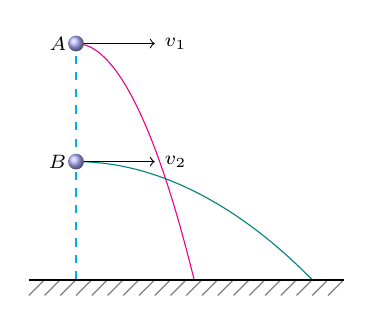
\begin{tikzpicture}[font=\scriptsize]
	\draw[magenta] (0,3) parabola bend(0,3) (1.5,0);
	\draw[teal] (0,1.5) parabola bend(0,1.5) (3,0);
	\draw[dashed,cyan] (0,0)--(0,3);
	\foreach \c/\a/\v in {(0,3)/A/v_1,(0,1.5)/B/v_2}{
		\draw[->] \c--++(1,0)node[right]{ \(\v\)};
		\shade[ball color=blue!30] \c node[left]{ \(\a\)} circle(.1);}
	\foreach \x in {-.6,-.4,...,3.4}
		\draw[gray] (\x,-.2)--++(.2,.2);
	\draw[thick] (-.6,0)--(3.4,0);
\end{tikzpicture}
\begin{choices}
	\item \(A\)、\(B\) 两球的初速度之比为 \(1:4\)
	\item \(A\)、\(B\) 两球下落过程中的动能变化量之比为\(1:2\)
	\item 若两球同时抛出，则落地的时间差为 $\sqrt{\dfrac{2h}{g}}$
	\item 若两球同时落地，则两球抛出的时间差为 $(\sqrt{2} - 1) \sqrt{\dfrac{2h}{g}}$
\end{choices}
\begin{answer}
	D\qquad 提示：
\end{answer}